
\begin{frame}
		\frametitle{Forces and Torques}
		\begin{figure}[p]
			\centering
			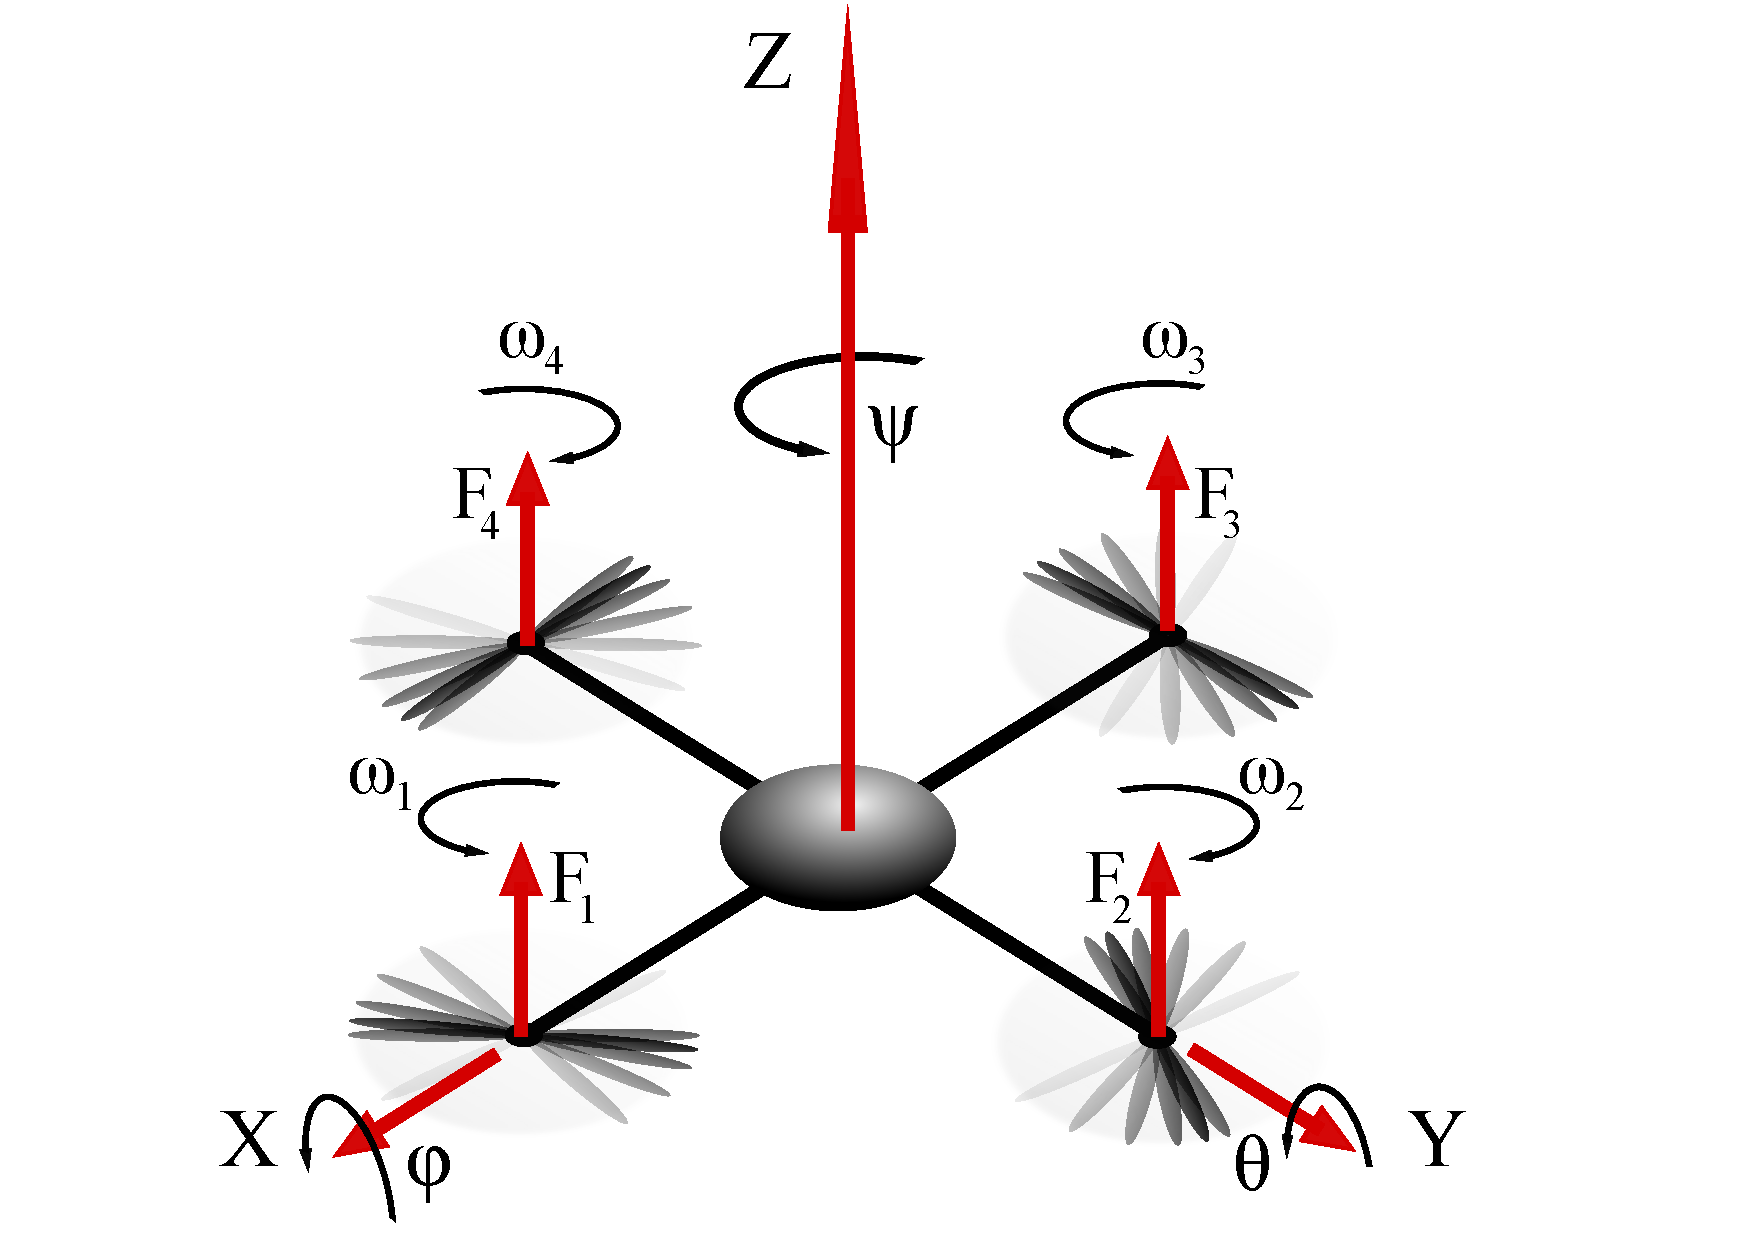
\includegraphics[width=0.8\textwidth]{images/Kraefte.pdf}
			\label{fig:Kraefte}
		\end{figure}
	\end{frame}

	\begin{frame}
		\frametitle{Newton-Euler Equations}
			\begin{columns}[T] % align columns
				\begin{column}{0.70\textwidth}
					Forces \\
					\[ F_{ext} = F_{g} + \sum_{i=1}^{4}{F_{i}} \]
					Torques \\
					\[ \tau_{ext} = \sum_{i=1}^{4}{\tau_{i}}+(\tau_{\varphi}+\tau_{\theta}) \]
				\end{column}
			\hfill
			\begin{column}{.25\textwidth}
				\begin{textblock}{0}(-2,1)
					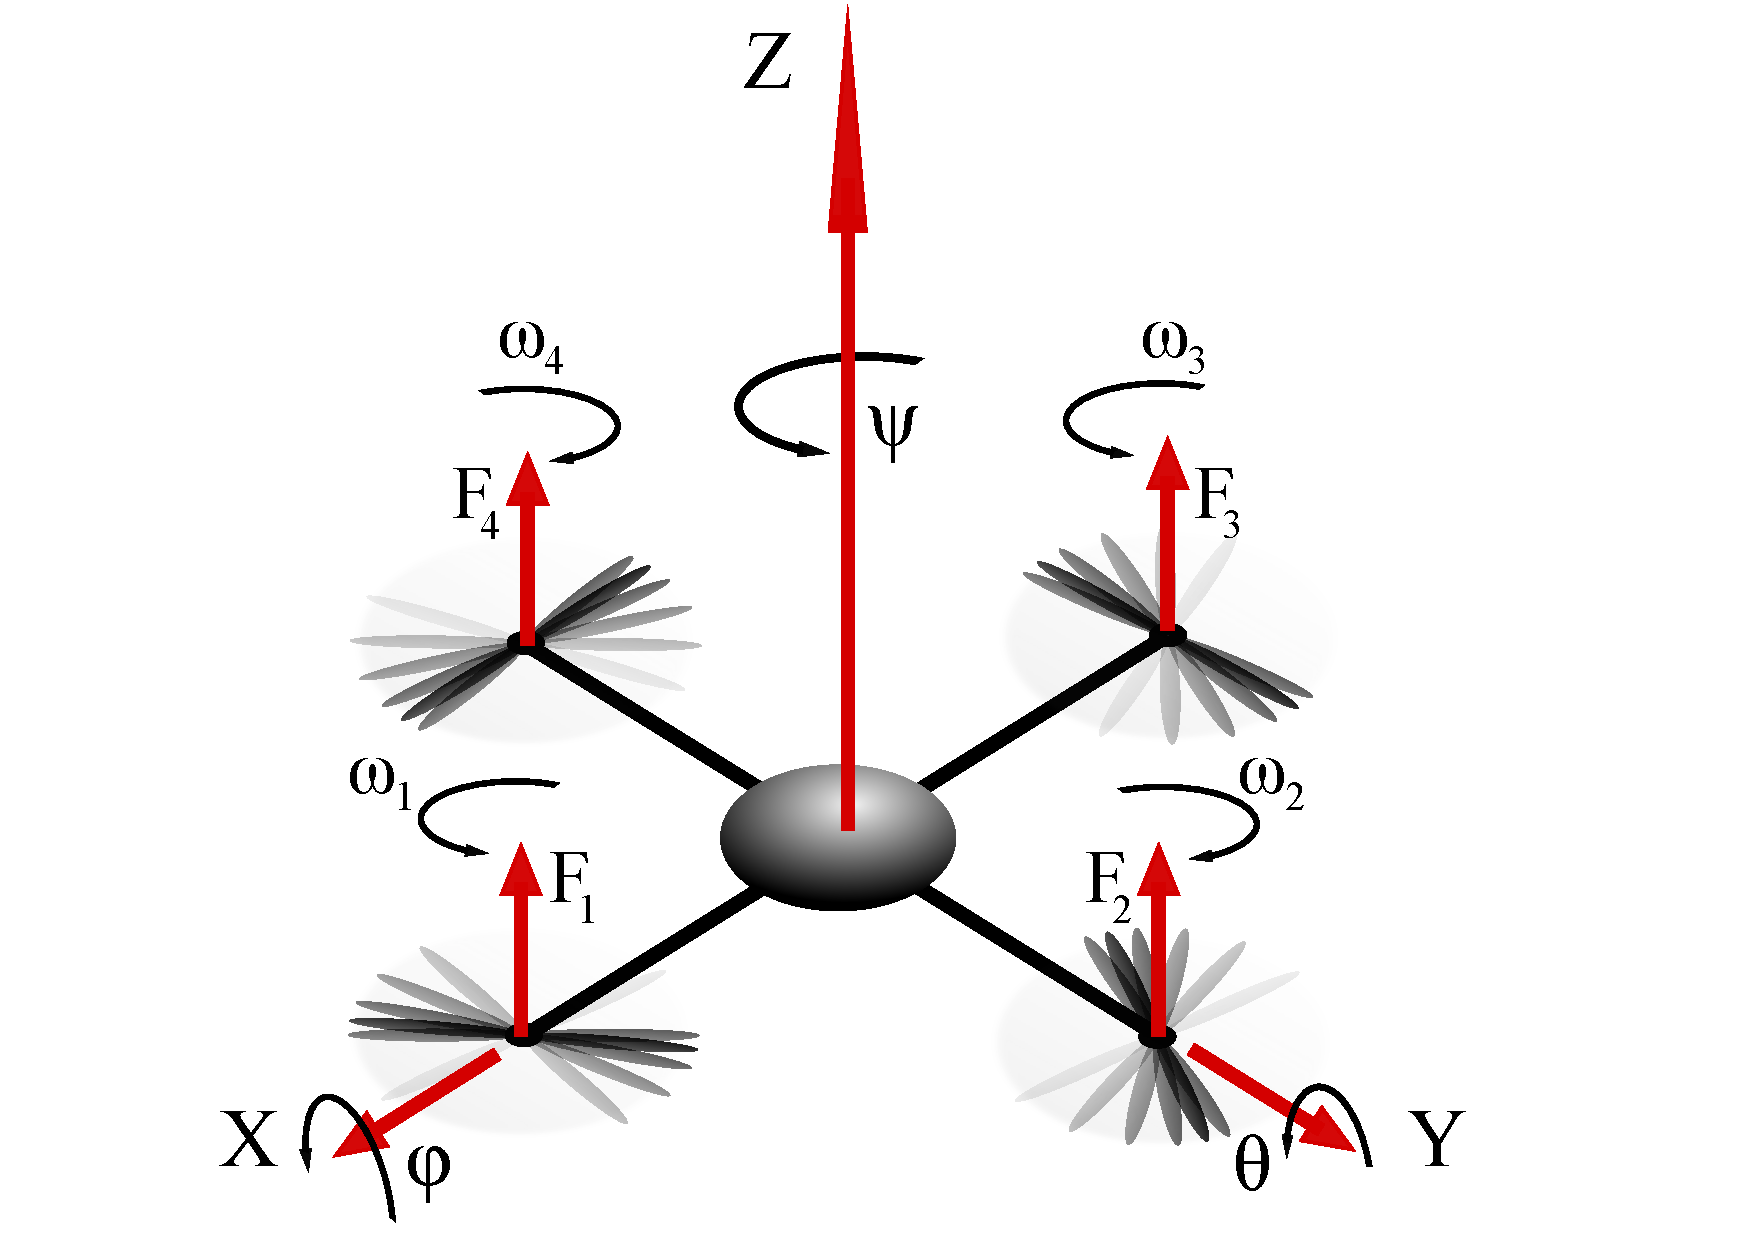
\includegraphics[width=5cm]{images/Kraefte.pdf}
					\label{fig:Kraefte klein}
				\end{textblock}
			\end{column}
		\end{columns}
	\end{frame}
		
	\begin{frame}
		\section{Model}
		\frametitle{Coordinate Systems}
			\begin{figure}[p]
				\centering
				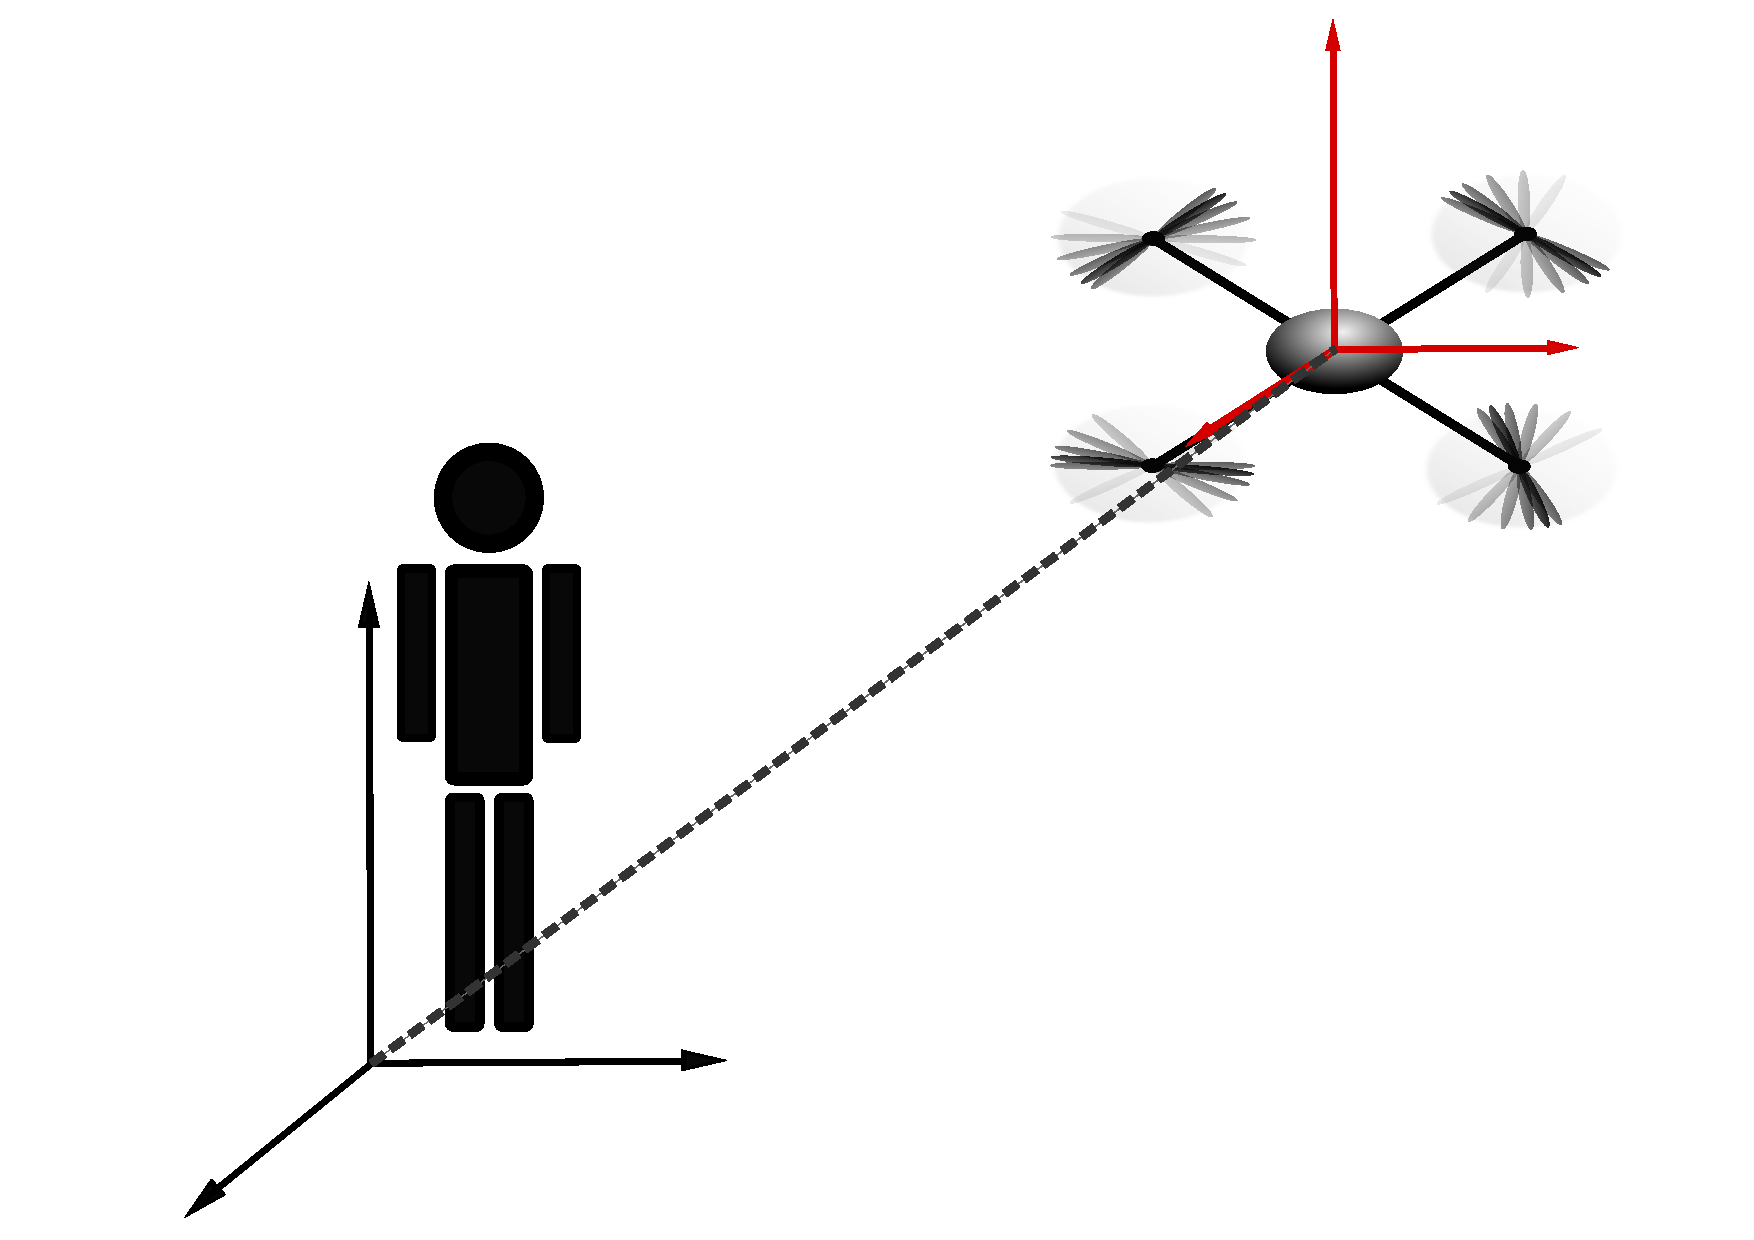
\includegraphics[width=0.8\textwidth]{images/Koordinatensysteme.pdf}
				\label{fig:Koordinatensysteme}
		\end{figure}
	\end{frame}

	
	\begin{frame}
		\frametitle{Quaternions}
		\begin{block}{}
			\[ q = a + \textup{i}b+\textup{j}c+\textup{k}d \qquad a, b, c, d \in \mathbb{R} \]
			\vspace{.1ex}
			\end{block}
			
			\vspace{1ex}
			\onslide<2-> representing rotation \( \Leftrightarrow \) \( \Vert q \Vert = 1 \) \\
			\vspace{1ex}			
			\onslide<3-> advantage \(\rightarrow\) no singularities \\
			\vspace{1ex}
			\onslide<4-> problem \(\rightarrow\) \( \Vert q \Vert = 1 \) additional constraint
	\end{frame}
	
	\begin{frame}
		\frametitle{Dynamics}
		Equations representing dynamics...
		\[ T(x, u) = M \cdot \begin{pmatrix} \dot{x}_{8} \\ \vdots \\ \dot{x}_{13} \end{pmatrix} + \Theta(x) \]
		\onslide<2->
		...expressed as system of differential equations:
		\[ \frac{\textup{d}}{\textup{d}t} 
			\begin{pmatrix}
						  x_{1} \\ \vdots \\ x_{7} \\ x_{8} \\ \vdots \\ x_{13}
			\end{pmatrix}
			=
			\begin{pmatrix}
							\dot{x}_{1} \\ \vdots \\ \dot{x}_{7} \\ M^{-1}(T(x,u)-\Theta(x))
			\end{pmatrix}
		\]
	\end{frame}
	
	\begin{frame}
		\frametitle{Prospect}
			Refinement of the model \\
			\vspace{1ex}
			\(\rightarrow\) wind \\
			\vspace{1ex}
			\(\rightarrow\) aerodynamical forces \\
	\end{frame}

%Der Befehl \include{datei} setzt dann hier die Datei datei.tex ,welche im selben Ordner liegt ein. Diese darf keinen Header enthalten
%\include{datei}